Let us consider a parameter t.\\ Considering the first equation:
 \begin{align}  \label{eq:solutions/line_plane/76/line_eq_1}
& \frac{x-5}{7} = \frac{y+2}{-5} = \frac{z}{1} = t
\end{align}
Line equation of \eqref{eq:solutions/line_plane/76/line_eq_1} can be written as,
 \begin{align} \label{eq:solutions/line_plane/76/line_eq_param}
& \myvec{x\\ y\\ z} = \myvec{7t+5\\ 5t-2\\ t} = \myvec{5\\ 2\\ 0} +t \myvec{7\\ -5\\ 1}
\end{align}
From \eqref{eq:solutions/line_plane/76/line_eq_param}, the direction vector is given by 
 \begin{align} \label{eq:solutions/line_plane/76/dir_vec_1}
\vec{d_1} = \myvec{7\\ -5\\ 1}
 \end{align}

Similarly, let us consider second equation:
 \begin{align} \label{eq:solutions/line_plane/76/line_eq_2}
& \frac{x}{1} = \frac{y}{2} = \frac{z}{3} = t
\end{align}
Line equation of  \eqref{eq:solutions/line_plane/76/line_eq_2} can be written as,
 \begin{align} \label{eq:solutions/line_plane/76/line_eq_param2}
& \myvec{x\\ y\\ z} = t \myvec{1\\ 2\\ 3}
\end{align}
From  \eqref{eq:solutions/line_plane/76/line_eq_param2},  the direction vector is given by 
 \begin{align} \label{eq:solutions/line_plane/76/dir_vec_2}
\vec{d_2} = \myvec{1\\ 2\\ 3}
 \end{align}
Two lines are perpendicular to each other when the dot product of their direction vectors is 0.\\
\\
Dot product of direction vectors $\vec{d_1}$ and $\vec{d_2}$ (from equation \eqref{eq:solutions/line_plane/76/dir_vec_1} and \eqref{eq:solutions/line_plane/76/dir_vec_2}) is given by:
 \begin{align}
& \vec{d_1}^T\vec{d_2}= (7 \times 1) + (-5 \times 2) + (1 \times 3) = 0   \label{eq:solutions/line_plane/76/dotproduct}\\
& \implies \boxed{\vec{d_1}^T\vec{d_2} = 0}  \label{eq:solutions/line_plane/76/res}
\end{align}


From \eqref{eq:solutions/line_plane/76/res}, as the dot product of direction vectors of the lines is 0 ($\vec{d_1^T}\vec{d_2}$ = 0), we can say that the lines are perpendicular to each other.

\renewcommand{\thefigure}{\arabic{figure}}
\begin{figure}[h!]
	\centering
	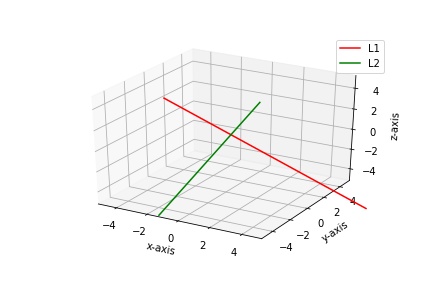
\includegraphics[width=\columnwidth]{./solutions/line_plane/76/lines.png}
	\caption{Lines perpendicular to each other}
	\label{myfig:solutions/line_plane/76/}
\end{figure}
